\documentclass[a4paper, 11pt, normalem]{article}

\usepackage{../../LaTeX-Templates/Notes}
\usepackage{subfiles}
\usepackage{adjustbox}

\title{The Little Crash Course of Particle Physics \vspace{-20pt}}
\author{Prof. Alex Lenz}
\date{\vspace{-15pt}Michaelmas 2019}
\rhead{\hyperlink{page.1}{Contents}}

\begin{document}

\maketitle

\section*{Meeting 10/10}
\textbf{\large QED:}
\begin{align}
    \La &= \bar{\psi}(i\cancel{\p}-m)\psi - \frac14F_{\mu\nu}F^{\mu\nu} \\
    \cancel{\p} &\to \cancel{D}: D_\mu = \p_\mu - ieA_\mu \\
    F_{\mu\nu} &= \p_\mu A_\nu - \p_\nu A_\mu
\end{align}

\textbf{\large Symmetry:}
\begin{align}
    \psi &\to e^{i\alpha}\psi \\
    A^\mu &\to A'^\mu = A^\mu + \p^\mu\alpha(x)
\end{align}
Known as a $U(1)$ local gauge symmetry, for EM. \\
Most accurate measurement in modern science is $(g-2)$ for the electron. 
Gone on to 5-loop now, $>10000$ diagrams to calculate that. 
\begin{table}[H]
    \centering
    \begin{tabular}{c|c|c|c}
        gauge & SU(N) & $N^2-1$ & N charges \\
        \hline
        strong & SU(3) & 8 gluons & 3 colours \\
        weak & SU(2) & $W^{+/-},Z^0$ & 2 charges \\
        (gravity) & & &
    \end{tabular}
\end{table}
\begin{align}
    \psi &\to \begin{cases} \begin{pmatrix} \psi_A \\ \psi_B \end{pmatrix} & \text{weak} \\ \begin{pmatrix} \psi_i \\ \psi_j \\ \psi_k \end{pmatrix} & \text{strong} \end{cases} & e^{i\alpha} &\to \begin{cases} e^{i\alpha_i\tau_i} & \text{weak, Pauli matrices, }i=1,2,3 \\ e^{i\alpha_i\lambda_i} & \text{strong, Gell-Mann matrices, }i=1,\dots,8 \end{cases}
\end{align}

The theoretical scattering rate of $B^- \to  K^-\mu^+\mu^-$ does not match that of experiment close enough that it can be simply down to innacuracies in experiment, so we posit a new boson, the \textit{Z'}, that could explain the difference between theory and experiment, and then we must find if such a boson can exist in harmony with the rest of the Standard Model.
\begin{equation}
    \text{\Large Exp} = \includegraphics[raise=-20pt]{bminus.pdf} + \includegraphics[raise=-20pt]{bminusprime.pdf}
\end{equation}  
Eq (7) shows the suggested sum, with the second diagram showing the new \textit{Z'} that may account for the difference. \\
For this \textit{Z'} to be the solution to the inconsistencies, it must also hold for all other couplings it could affect in the Standard Model.

\section*{Meeting 17/10}
\textit{Taken by Aleksey this week, just a few maths notes.}
\begin{align}
    F_{\mu\nu} &= D_\mu A_\nu - D_\nu A_\mu \\
               &= (\p_\mu - igA_\mu)A_\nu - (\p_\nu - igA_\nu)A_\mu \\
               &= \p_\mu A_\nu - \p_\nu A_\mu - ig[A_\mu,A_\nu] \\
    A_\mu &= \sum_{a=1}^{n^2-1} A_\mu^at^a,~ SU(n) \\
    U(1) &\implies [A_\mu,A_\nu] = 0 
\end{align}
Of course, for the other symmetry groups used in SM, this commutator will not be zero, as Eq (11) implies, which leads to the more complicated Lagrangian for these theories. 
The basic formulation for proving gauge invariance of each group is the same, and follows below, but for the SU(2) and SU(3) groups, Eq (11) must be remembered and applied in addition to the usual methods. 
\begin{align}
    \psi(x) \to \psi'(x) &= e^{ig\alpha(x)} \\
    A_\mu \to A_\mu' &= A_\mu + \p_\mu\alpha(x) \\
    \La &= -\frac14 F_{\mu\nu}F^{\mu\nu} + \bar{\psi}(i\p_\mu\gamma^\mu - m)\psi \\
    \p_\mu \to D_\mu &= \p_\mu - igA_\mu 
\end{align}
All of this is then mashed together into the SM Lagrangian,
\begin{align}
    \La^{SM} &= -\frac14 F_{\mu\nu}F^{\mu\nu}~ \to \text{gauge term} \\ 
             &+ i\bar{\psi}\cancel{D}\psi ~ \to \text{Fermion term} \\
             &+ (D_\mu\phi)^\dagger(D^\mu)\phi - V(\phi) ~ \to \text{Higgs term} \\
             &- Y_{ij}\bar{\psi}_i\phi\psi_j + h.c. ~ \to \text{Yukawa term} \\
             & SU_c(3)\otimes SU(2)_L\otimes U(1)
\end{align}
Very reduced form, most terms can be largely expanded, i.e.
\begin{align}
    -\frac14 F_{\mu\nu}F^{\mu\nu} &= \underbrace{-\frac14 G_{\mu\nu}G^{\mu\nu}}_{SU_c(3)} - \underbrace{\frac14 F_{\mu\nu}F^{\mu\nu}}_{SU(2)_L} - \underbrace{\frac14 B_{\mu\nu}B^{\mu\nu}}_{U(1)} \\
    G_{\mu\nu} &= D_\mu A_\nu - D_\nu A_\mu \\
    D_\mu &= \p_\mu - igA_\mu,\; A_\mu = \frac12 A_\mu^a\lambda^a,\; a = 1,\dots,8 \\
    [A_\mu^a\lambda^a,A_\nu^a\lambda^a] &\neq 0
\end{align}

\section{Meeting 24/10}
Now that we're comprehending the gauge invariance of SU(N) Lagrangians, moving on. 
\begin{align}
    \La = \bar{\psi}(i\cancel{D}-m)\psi - \frac14 F_{\mu\nu}F^{\mu\nu}
\end{align}
Gauge symmetry thus far has been relatively straightforward, but the mass terms cause some problems.
\begin{enumerate}
    \item Spontaneous Symmetry Breaking: We start off by discussing the issues with the mass terms in these theories, how they initially to symmetry breaking and parity violation of the weak force. 
        \begin{itemize}
            \item $m_A^2A_\mu A^\mu$ - bosons
            \item $m\bar{\psi}\psi$ - fermions
        \end{itemize}
        Introducing the concept of right- and left-handed particles can resolve some of these issues within electroweak theory, where left-handed particles transform under SU(2) space, and right-handed particles transform as a number, so do not transform under the weak interaction. 
        \begin{align}
            \psi &= \underbrace{\psi_L}_{SU(2)_L} + \underbrace{\psi_R}_{\land} = \frac{1-\gamma_5}{2}\psi + \frac{1+\gamma_5}{2}\psi \\
            \implies m\bar{\psi}\psi &= m\left(\bar{\psi}_L\psi_R + \bar{\psi}_R\psi_L\right)
        \end{align}
        So including right-handed fermions in the mass term leads to no gauge invariance(?). 
        Including spontaneous symmetry breaking into the theory can account for this (?) - but the SM still has SU(2)$_L$ space.
    \item Quantum Field Theory: A possible explanation used to recapture mass terms into gauge invariant lagrangian was from something called \emph{renormalisation.} 
        Every interaction is not a single Feynman diagram, but an infinite sum of all possible valid interactions, even for just $\psi\to\psi$. \\
        \textit{doodle diagrams}\\
        Attempting to calculate for a single diagram would result in an infinity, or even a single vertex, but taking the entire sum will lead to a finite result. 
        People proved this in the 70s as true for any gauge field theory(?) which is why like them so much and still use them. 
\end{enumerate}
Higgs mechanism:
\begin{itemize}
    \item sorts out $m\psi,mA$ issues
    \item gauge symmetry and field theory - renormalisable and stuff
    \item Only really issue with it was that it predicted a particle to explain it that hadn't been seen before, until 2012, then everyone was happy, \textit{doodle mechanism}
\end{itemize}
\begin{multicols}{2}
Higgs - $\phi \in$ SU(2)$_L$:
\begin{align}
    (D_\mu\phi)(D^\mu\phi)^\dagger &- V(\phi,\phi^\dagger) \\
    \langle\phi\rangle &= \begin{pmatrix} 0 \\ v\end{pmatrix}
\end{align}
    \begin{figure}[H]
    \centering
    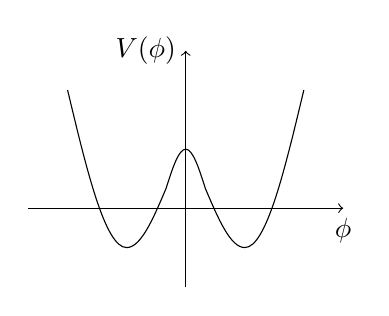
\begin{tikzpicture}
        \draw[->] (-2,0) -- (2,0) node[anchor=north] {$\phi$};
        \draw[->] (0,-1) -- (0,2) node[anchor=east] {$V(\phi)$};
        \draw (-1.5,1.5) sin (-0.75,-0.5) cos (-0.25,0.25) sin (0,0.75) cos (0.25,0.25) sin (0.75,-0.5) cos (1.5,1.5);
    \end{tikzpicture}
\end{figure}
\end{multicols}
In the early universe, so high energy that the Higgs mechanism resembled a simple $x^2$ potential around $\phi=0$, but as the universe cooled, the symmmetry broke into the double-welled potential shown above. 
This is developed using Goldstone's theorem, akin to symmetry breaking in ferromagnets.
\begin{align}
    \La &= \frac12\p_\mu\phi\p^\mu\phi - \left(\frac12\mu^2\phi^2 + \frac14\lambda\phi^4\right)
\end{align}
In this Lagrangian, setting $\mu^2>0$ corresponds to a potential well around $\phi=0$ as would be seen in the early universe, but there is no reason for $\mu^2>0$, so must also look at $\mu^2<0$, where you get the double well above and a Goldstone boson can be found.
\begin{align}
    (\p_\mu + igA_\mu)\begin{pmatrix} 0 \\ v\end{pmatrix} (\p^\mu + igA^\nu)\begin{pmatrix}v \\ 0\end{pmatrix} &= \dots + \underbrace{g^2v^2}_{m_A^2}A_\mu A^\nu \\
    g\bar{\psi}_L\phi\psi_R \to g\bar{\psi}_L\begin{pmatrix} 0\\ v\end{pmatrix} \psi_R &= gv\bar{\psi}_L\psi_R
\end{align}








\end{document}












